\section{Implementation}
We will describe here the multiple choices that have been made during this project, and the reason behind these choices, as well as the result of our implementation.

\subsection{Chosen display techniques}
There are multiple factors to take into account : 
\begin{enumerate}
\item The availability of the technology.
\item The potential price of the required materials.
\item The time to setup the display.
\item The scaling for a medium-sized audience.
\item The compatibility with the double requirement : a view for the performer, and another for the spectators.
\end{enumerate}

We are now going to study these requirements point by point.
\subsubsection{Availability}
This is the main problem : many of the display devices presented in \ref{chap:3ddisp} have only been the subject of research and not of a real implementation sold by a company (e.g. holograms). Also, the development state of some technologies  might not be sufficient for what we are striving for (e.g. autostereoscopic displays which are only present in very small screens like smartphones).
\subsubsection{Price}
Some technologies might be irrelevant only because of the amount of money needed to get a working implementation. For instance, an active 84" 3D HDTV generally costs more than ten thousand dollars, which is unsuitable to this project.
\subsubsection{Setup time}
Some methods might require a very long time to setup. While we don't have a required maximum time to setup the show, we should try to keep it as low as possible. For instance, the Pepper's Ghost technique is quite long to setup, because there is a lot of massive hardware, videoprojectors, screens, to setup.
\subsubsection{Scaling}
Since this is for a show, we need a system that will allow everybody in the room to enjoy the performance. The estimate is at about 40 persons : we need a display that provides big enough viewing angles and is big enough for everybody to be able to enjoy it. A square display with a side of two meters would be ideal to enable complete immersion.
\subsubsection{Double-view requirement}
This is one of the hardest requirements, because it can easily double the quantity of required hardware. For instance, if we were to use 3D TVs, we would need one TV for the viewers and one for the performer.

\subsubsection{The choice}
We chose to go with the Pepper's Ghost technique, with polarized stereo glasses. This was mainly because it was the only method efficiently available with all the tools at our disposal : no additional fees are required.

Due to computer limits, we could not test the two views, but it is implemented in our software. We mainly did focus on the Aerial Percussion, because we did not know how to use the DRILE code. 

\subsection{Aerial Percussion implementation}
We will described here the implementation of the Aerial Percussion 3D renderer.

\begin{figure}[h!]
\centering
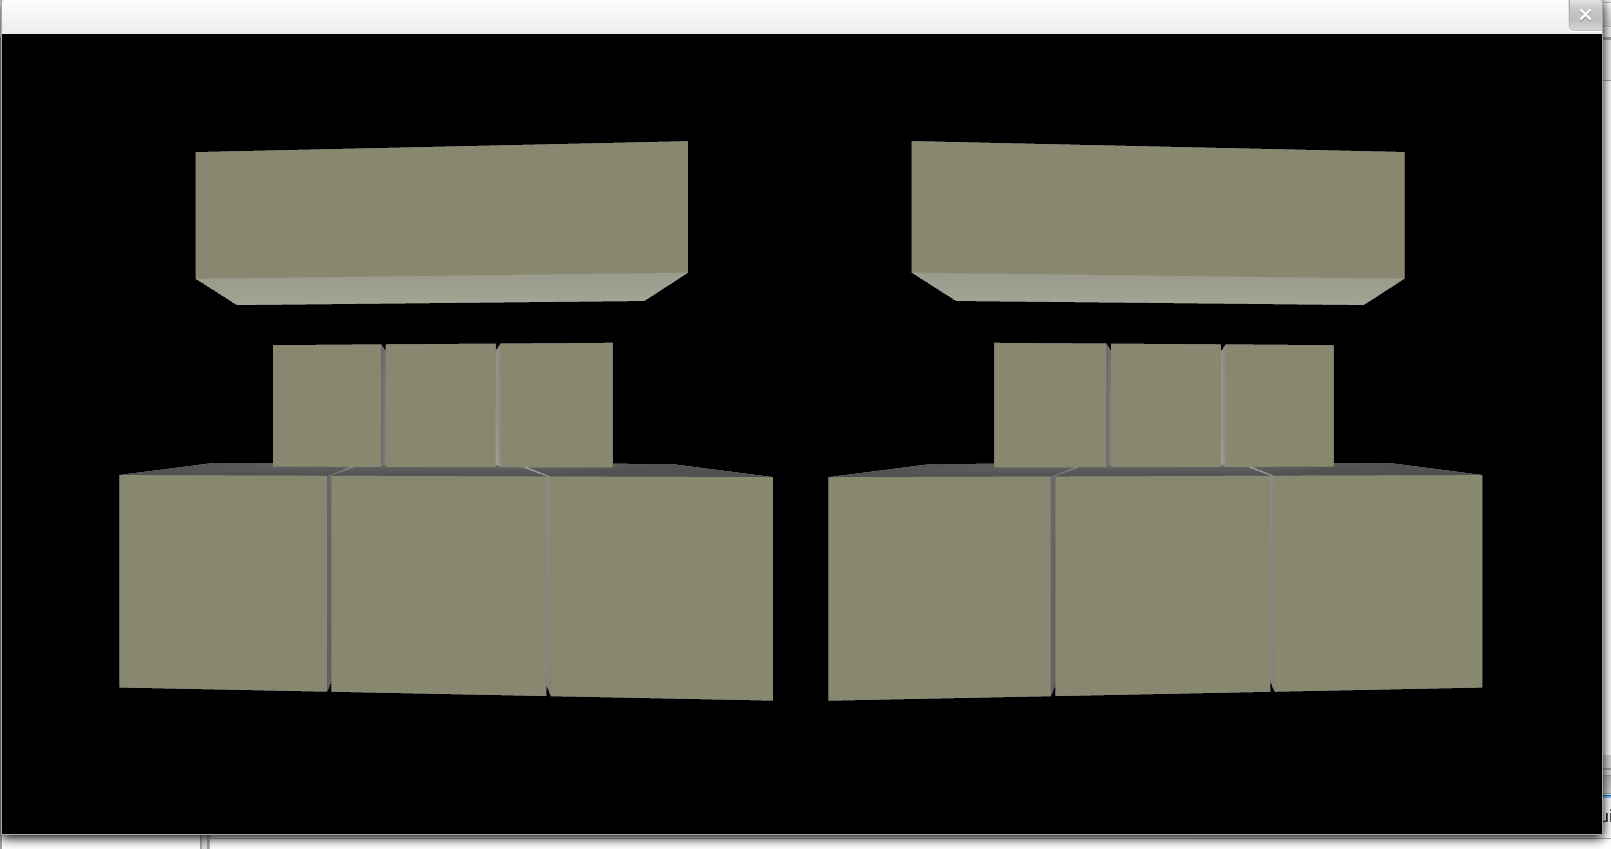
\includegraphics[scale=0.3]{image/percuScreen.png}
\caption{A screenshot of the Aerial Percussion renderer}
\label{fig:percScreen}
\end{figure}

\subsubsection{Technologies used}
We worked with \brand{OpenFrameworks}, a \brand{C++} abstraction over many different media libraries, like \brand{OpenGL}, \brand{OpenNI} and many others. It makes the implementation of creative software easy while retaining the power and speed efficiency of the \brand{C++}.

Our software listens to \brand{OSC} messages, which means that it would be easy to put it on two computers and have one computer display the images for the spectators, and the other for the musician.

\subsubsection{Displaying the data}
\paragraph{Pepper's Ghost technique}
In order to have the Pepper's Ghost technique work efficiently, we have to display our shapes on a black background, so that only the bright parts reflects on the glass screen.

\paragraph{Stereoscopic display}
The method uses two projectors, one on the top of another.
Each projector has a polarizing filter and is connected to a different input of the computer.

The computer, running \brand{Debian GNU/Linux}, is set up so that there is a single viewport of twice a projector's horizontal resolution. Each projector receives one half of the viewport.

For instance, the actual resolution of a projector is $1920 \times 1080$. Hence, the viewport is $3840 \times 1080$.

The software then runs at the same resolution, and the image is displayed from two point of views, that slightly differs on the horizontal axis, as shown on figure \ref{fig:percScreen}. We used frame-buffer objects to achieve this. This allows to generate a 3D effect when the images are projected on the same point in space by the dual projector system, because each eye will receive the correct image, as we could see on paragraph \ref{par:polarized}.

\subsubsection{Additional features}
We added the feature to change the distance between the eyes in order to find the most pleasant one, using the left and right keyboard keys.
We can also zoom in and out using the up and down keys.

The space key will change the point of view from front to back.

The software also reacts by changing the color of a box when the musician puts a drumstick inside a virtual drum element.

